\usetikzlibrary{automata, positioning}
\smalltitle{سوال 4}
\begin{latin}
  \noindent
  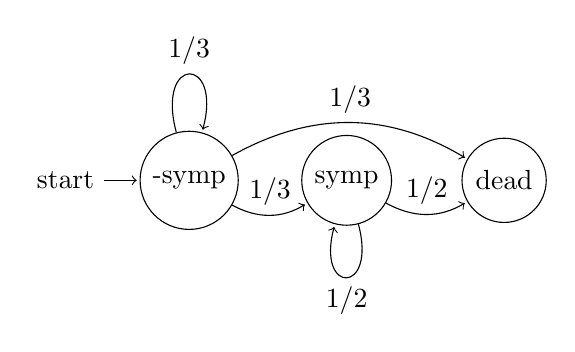
\begin{tikzpicture}[shorten >=1pt, node distance=2cm, on grid, auto]
    \node[state, initial] (q0) {-symp};
    \node[state] (q1) [right=of q0] {symp};
    \node[state] (q2) [right=of q1] {dead};
 
    \path[->]
    (q0) edge [bend right] node {1/3} (q1)
    (q0) edge [bend left] node {1/3} (q2)
    (q0) edge [loop above] node {1/3} (q0)
    (q1) edge [bend right] node {1/2} (q2)
    (q1) edge [loop below] node {1/2} (q1);
    % (q2) edge [loop above] node {1} (q2);
 \end{tikzpicture}
 \begin{equation*}
   \begin{matrix}
         &-symp&symp&dead\\\\
    -symp&\frac{1}{3}&\frac{1}{3}&\frac{1}{3}\\
    symp&0&\frac{1}{2}&\frac{1}{2}\\
    dead&0&0&1
  \end{matrix}
 \end{equation*}
\noindent
 $\pi_{-symp} = 1/3*\pi_{-symp}$\\\\
 $\pi_{symp} = 1/3*\pi_{-symp} + 1/2 *\pi_{symp}$\\\\
 $\pi_{dead} = 1/3 * \pi_{-symp} + 1/2 *\pi_{symp} + \pi_{dead}$\\\\
 $\pi_{dead} + \pi{symp}+\pi_{-symp} = 1 \xrightarrow[]{} \pi_{dead} = 1,\pi_{symp} = \pi_{-symp} = 0$
 \begin{center}
  As we have seen, in infinity, the patient would likely(prob = 1) be dead.
 \end{center}
 \noindent
 $E(-symp) = 1 + 1/3 * E(-symp) + 1/3 * E(symp) + 1/3 * E(dead)$\\\\
 $E(symp) = 1 + 1/2 * E(symp) + 1/2 * E(dead)$\\\\
 $E(dead) = 0$\\\\
 Now we solve the equations to find our expected values.\\
 $E(symp) = 1 + 1/2 * E(symp) \rightarrow E(symp) = 2$\\\\
 $E(-symp) = 1 + 1/3 * E(-symp) + 1/3 * 2 \rightarrow E(symp) = 5/2$\\\\
 This means if we start with no syptom and each transition between states takes 1 day, the patient will likely die in 5/2 days.
\end{latin}